\documentclass[11pt, oneside]{article} 
\usepackage{geometry}
\geometry{letterpaper} 
\usepackage{graphicx}
	
\usepackage{amssymb}
\usepackage{amsmath}
\usepackage{parskip}
\usepackage{color}
\usepackage{hyperref}

\graphicspath{{/Users/telliott_admin/Tex/png/}}
% \begin{center} 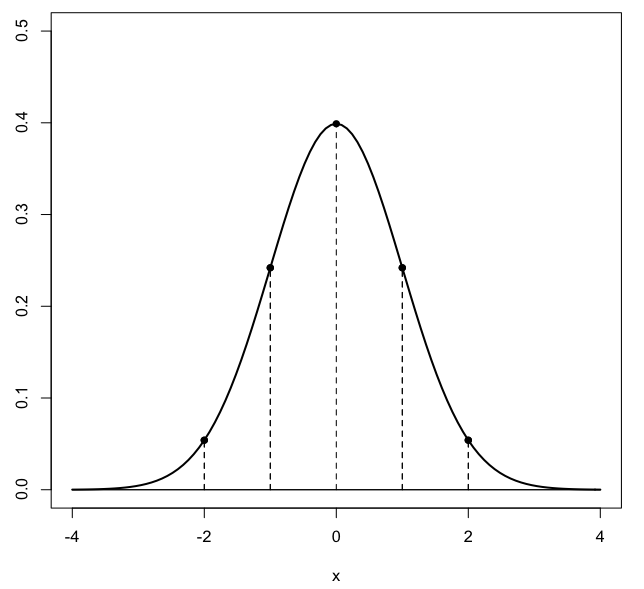
\includegraphics [scale=0.4] {gauss3.png} \end{center}

\title{Newton and the binomial}
\date{}

\begin{document}
\maketitle
\Large

\subsection*{standard binomial}

As you know, the binomial expansion for the first few positive integers $n$ is
\[ (a+b)^1 = a + b \]
\[ (a+b)^2 = a^2 + 2ab + b^2 \]
\[ (a+b)^3 = a^3 + 3a^2b + 3ab^2 + b^3 \]
\[ (a+b)^4 = a^4 + 4a^3b + 6a^2b^2 + 4ab^3 + b^4 \]

\[ (a + b)^n = \sum_{k=0}^{k=n} c_k \ a^{n-k} b^{k} \]
The coefficients $c_k$ are given by Pascal's triangle or by computing
\[ \binom{n}{k} = \frac{n!}{k!(n-k)!}  \]
For 
\[ k = 0, \ \ \ \ \frac{n!}{0!(n-0)!} = 1 \]
\[ k = 1, \ \ \ \ \frac{n!}{1!(n-1)!} = n \]
\[ k = 2, \ \ \ \ \frac{n!}{2!(n-2)!} = \frac{n(n-1)}{2!} \]
\[ k = 3, \ \ \ \ \frac{n!}{3!(n-3)!} = \frac{n(n-1)(n-2)}{3!} \]
This can also be written as
\[ = \frac{n}{1} \cdot \frac{(n-1)}{2} \cdot \frac{(n-2)}{3} \]

Let us just consider binomials of the form $a = 1$, so then substitute $x$ for $b$
\[ (1 + x)^n = \sum_{k=0}^{k=n} c_k \ x^k \]

The expansion becomes ($x^0 = 1$)
\[ 1 + n \cdot x + n \cdot \frac{(n-1)}{2} \cdot x^2 + \frac{n}{1} \cdot \frac{(n-1)}{2} \cdot \frac{(n-2)}{3} \cdot x^3 + \dots \]

This series terminates when $n = k$, and the coefficients are symmetric about $k=n/2$.  If $n$ is even, the two middle terms of the sequence are equal.

Now, the natural question is, what will happen if we substitute $r$ for $n$, where is $r$ is a rational exponent, or may even be negative?

\subsection*{Newton}

Newton wrote the binomial expansion in this way
\[ (P + PQ)^{m/n} = P^{m/n} + \frac{(m)}{(n)}P^{m/n}Q + \frac{(m)}{(n)}\frac{(m-n)}{(2n)}P^{m/n}Q^2 + \cdots \]
\[ + \frac{(m)}{(n)}\frac{(m-n)}{(2n)}\frac{(m-2n)}{(3n)}P^{m/n}Q^3 + \cdots \] 

This looks a little strange to modern eyes, but it's actually the same as the standard binomial. 

Notice that we can factor out $P^{m/n}$ so
\[ (1 + Q)^{m/n} = 1 + \frac{(m)}{(n)} Q  + \frac{(m)}{(n)} \frac{(m-n)}{(2n)} Q^2 + \frac{(m)}{(n)} \frac{(m-n)}{(2n)} \frac{(m-2n)}{(3n)} Q^3 + \cdots \] 
Then just bring $n$ up into the numerator
\[ (1 + Q)^{m/n} = 1 + \frac{m/n}{1} Q  + \frac{(m/n)}{1} \frac{(m/n-1)}{2} Q^2 + \]
\[ + \frac{(m/n)}{1} \frac{(m/n-1)}{2} \frac{(m/n-2)}{3} Q^3 + \cdots \] 
Substitute $r$ for $m/n$
\[ (1 + Q)^r = 1 + r Q  + r \frac{(r-1)}{2} Q^2 + r \frac{(r-1)}{2} \frac{(r-2)}{3} Q^3 + \cdots \] 

This is the binomial with $x = Q$.

One difference is that Newton used it for negative integers and even for a fractional power.  A key change is that in these cases the series becomes infinite.

\subsection*{usage}
We can use this to compute roots.  Suppose $Q = 1$ and $r = 1/3$, so we are looking for the cube root of $2$.  The terms of the series are $1 + 1/3 + \dots$

\[ \frac{1}{3} \cdot \frac{-2/3}{2} = - \frac{1}{3^2} \]
\[ - \frac{1}{3^2} \cdot \frac{-5/3}{3} = \frac{5}{3^4} \]
\[  \frac{5}{3^4} \cdot \frac{-8/3}{4} = -\frac{10}{3^5} \]
\[ -\frac{10}{3^5} \cdot \frac{-11/3}{5} = \frac{22}{3^6} \]
\[  \frac{22}{3^6} \cdot \frac{-14/3}{6} = \frac{154}{3^8} \]
\[ .. \]


\[ = 1 + \frac{1}{3} - \frac{1}{9} + \frac{5}{81} - \frac{10}{243} + \frac{22}{729} - \frac{154}{6561} \dots  \]
which seems pretty close (but not that close) to $1.259921$.

Another use is to obtain a series for $1/(1+x)$.
\[ (1 + Q)^r = 1 + rQ + r\frac{(r-1)}{2}Q^2 + r\frac{(r-1)}{2}\frac{(r-2)}{3}Q^3 + \cdots \]
\[ (1+x)^{-1} = 1 - x + x^2 - x^3 + x^4 + \cdots  \]

Newton checked this by multiplying:
\[ 1 = (1+x)(1 - x + x^2 - x^3 + x^4 + \cdots)  \]

And if you know that the area under this curve is the logarithm, you can integrate the series for $1/(1+x)$ to obtain
\[ \ln(1+x) = x - \frac{x^2}{2} + \frac{x^3}{3} - \frac{x^4}{4} + \cdots \]
The logarithms obtained by this method can be easily verified.

\subsection*{derivation}
So far as I know Newton did not provide a proof of his version of the binomial theorem.  I found a discussion of how he came to it here:

\url{http://www.quadrivium.info/MathInt/Notes/NewtonBinomial.pdf}

\begin{center} 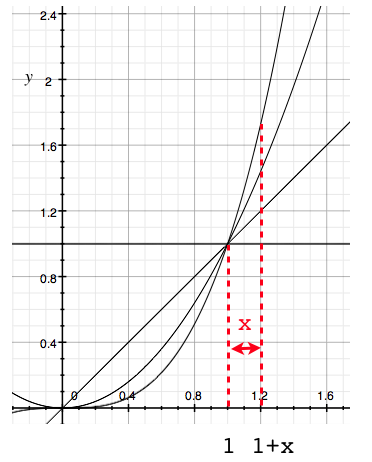
\includegraphics [scale=0.5] {newton1.png} \end{center}
Following Wallis, Newton studied expressions for the area under various curves.  

\subsection*{powers of x}

Above: $y=x^n, n = \{0,1,2\}$.  These areas were apparently known prior to Newton, and I am not sure exactly how this was done, but I will use results obtained by integration.

It's perhaps a little confusing, but we use $x$ here for two purposes.  First, the curves are $f(x)=x^n$. Second, we seek the area under each of these curves between the endpoints $1$ and $1+x$.  So for each $n$, we will compute the integral of $x^n$ and evaluate that between the limits $1$ and $1+x$.

$\circ$  For $y = x^0 = 1$, the area under the curve is just $x \cdot 1 = x$.

$\circ$  For $y = x$, the area under the curve is
\[ \frac{x^2}{2} \ \bigg |_1^{1+x} = \frac{(1+x)^2 - 1}{2}  = \frac{2x + x^2}{2} = x + \frac{x^2}{2} \]

$\circ$  For $y = x^2$, the area under the curve is
\[ \frac{x^3}{3} \ \bigg |_1^{1+x} = \frac{(1+x)^3 - 1}{3}  = \frac{3x + 3x^2 + x^3}{3} \]
\[ = x + x^2 + \frac{x^3}{3}  \]

$\circ$  For $y = x^3$, the area under the curve is
\[ \frac{x^4}{4} \ \bigg |_1^{1+x} = \frac{(1+x)^4 - 1}{4}  = \frac{4x + 6x^2 + 4x^3 + x^4}{4} \]
\[ = x + \frac{3}{2} x^2 + x^3 + \frac{x^4}{4}  \]
which we can write as 
\[ = x + \frac{3}{2} x^2 + \frac{3}{3} x^3 + \frac{x^4}{4}  \]

$\circ$  For $y = x^4$, the area under the curve is
\[ \frac{x^5}{5} \ \bigg |_1^{1+x} = \frac{(1+x)^5 - 1}{5}  \]
\[ = \frac{5x + 10x^2 + 10x^3 + 5x^4 + x^5}{5} \]
\[ = x + 2 x^2 +  2 x^3 + x^4 + \frac{x^5}{5}  \]
which we can write as 
\[ x + \frac{4}{2}x^2 + \frac{6}{3}x^3 + \frac{6}{4}x^4 + \frac{1}{5}x^5 \]

$\circ$  For $y = x^5$, we would find
\[ x + \frac{5}{2}x^2 + \frac{10}{3}x^3 + \frac{10}{4}x^4 + \frac{5}{5}x^5 + \frac{1}{6}x^6 \]

If we look carefully at what we've obtained, we see that there is a sum of terms like $x^p/p$ times a cofactor which goes like Pascal's triangle or a standard binomial expansion (and indeed, that's where it came from).  Newton organized the cofactors into a table.

\subsection*{table}

\[
\begin{matrix}
\text{p}  \\
x/1  \\
x^2/2 \\
x^3/3 \\
x^4/4 \\
x^5/5 \\
x^6/6 \\
x^7/7
\end{matrix} \ \ \ \
\begin{matrix}
0 & 1 & 2 & 3 & 4 & 5  \\
1 & 1 & 1 & 1 & 1 & 1  \\
0 & 1 & 2 & 3 & 4 & 5 \\
0 & 0 & 1 & 3 & 6 & 10 \\
0 & 0 & 0 & 1 & 4 & 10 \\
0 & 0 & 0 & 0 & 1 & 5 \\
0 & 0 & 0 & 0 & 0 & 1 \\
0 & 0 & 0 & 0 & 0 & 0
\end{matrix}
\]

That is, we have for $x^2$ that the area is
\[ (1)x + (2)\frac{1}{2}x^2 + (1)\frac{1}{3}x^3 = x + x^2 + \frac{1}{3}x^3 \]

Newton noticed (as did Pascal) that the pattern of coefficients can be generated by addition.  For example, the $6$ in the column for $n=4$ is generated by adding together the entry to its immediate left ($3$), plus the entry above that (also $3$).  Thus, having the first row (all $1$), and the column under $n=0$, one can generate the rest of the table mechanically.

Now, Newton says, what happens if we add an additional column for $n=-1$, and we make a rule that the entry in the first row must be $1$, because all the other columns have this value.

\[
\begin{matrix}
\text{p}  \\
x/1  \\
x^2/2 \\
x^3/3 \\
x^4/4 \\
x^5/5 \\
x^6/6 \\
x^7/7
\end{matrix} \ \ \ \
\begin{matrix}
-1 & 0 & 1 & 2 & 3 & 4 & 5  \\
\ \ 1 & 1 & 1 & 1 & 1 & 1 & 1  \\
\ \ . & 0 & 1 & 2 & 3 & 4 & 5 \\
\ \ . & 0 & 0 & 1 & 3 & 6 & 10 \\
\ \ . & 0 & 0 & 0 & 1 & 4 & 10 \\
\ \ . & 0 & 0 & 0 & 0 & 1 & 5 \\
\ \ . & 0 & 0 & 0 & 0 & 0 & 1 \\
\ \ . & 0 & 0 & 0 & 0 & 0 & 0
\end{matrix}
\]

How do we fill  in the missing entries?  By using the addition rule!  The first missing value must be a $-1$, so that it plus the $1$ above add together to give the $0$ to its right.
\[
\begin{matrix}
\text{p}  \\
x/1  \\
x^2/2 \\
x^3/3 \\
x^4/4 \\
x^5/5 \\
x^6/6 \\
x^7/7
\end{matrix} \ \ \ \
\begin{matrix}
-1 & 0 & 1 & 2 & 3 & 4 & 5  \\
\ \ 1 & 1 & 1 & 1 & 1 & 1 & 1  \\
-1 & 0 & 1 & 2 & 3 & 4 & 5 \\
\ \ . & 0 & 0 & 1 & 3 & 6 & 10 \\
\ \ . & 0 & 0 & 0 & 1 & 4 & 10 \\
\ \ . & 0 & 0 & 0 & 0 & 1 & 5 \\
\ \ . & 0 & 0 & 0 & 0 & 0 & 1 \\
\ \ . & 0 & 0 & 0 & 0 & 0 & 0
\end{matrix}
\]
He filled out the rest of the column for $n=0$ using this idea.  
\[
\begin{matrix}
\text{p}  \\
x/1  \\
x^2/2 \\
x^3/3 \\
x^4/4 \\
x^5/5 \\
x^6/6 \\
x^7/7
\end{matrix} \ \ \ \
\begin{matrix}
-1 & 0 & 1 & 2 & 3 & 4 & 5  \\
\ \ 1 & 1 & 1 & 1 & 1 & 1 & 1  \\
-1 & 0 & 1 & 2 & 3 & 4 & 5 \\
\ \ 1 & 0 & 0 & 1 & 3 & 6 & 10 \\
-1 & 0 & 0 & 0 & 1 & 4 & 10 \\
\ \ 1 & 0 & 0 & 0 & 0 & 1 & 5 \\
-1 & 0 & 0 & 0 & 0 & 0 & 1 \\
\ \ 1 & 0 & 0 & 0 & 0 & 0 & 0
\end{matrix}
\]
This gives the series for $1/(1+x)$ that we have above.  
\[ \frac{1}{1+x} = 1 - x + x^2 - x^3 + x^4 + \dots  \]
One can check that it's correct by multiplying out.
\[ 1 = 1 - x + x - x^2 + x^2 - x^3 + x^3 - x^4 + x^4 + \dots  = 1 \]
Using this idea, one can fill in the table for the negative integers.  In particular, the column for $-2$ is
\[
\begin{matrix}
\text{p}  \\
x/1  \\
x^2/2 \\
x^3/3 \\
x^4/4 \\
x^5/5 \\
x^6/6 \\
x^7/7
\end{matrix} \ \ \ \
\begin{matrix}
 -2 & -1 & 0 & 1 & 2 & 3 & 4 & 5  \\
\ \ 1 & \ \ 1 & 1 & 1 & 1 & 1 & 1 & 1  \\
-2 & -1 & 0 & 1 & 2 & 3 & 4 & 5 \\
\ \ 3 & \ \ 1 & 0 & 0 & 1 & 3 & 6 & 10 \\
-4 & -1 & 0 & 0 & 0 & 1 & 4 & 10 \\
\ \ 5 & \ \ 1 & 0 & 0 & 0 & 0 & 1 & 5 \\
-6 & -1 & 0 & 0 & 0 & 0 & 0 & 1 \\
\ \ 7 & \ \ 1 & 0 & 0 & 0 & 0 & 0 & 0
\end{matrix}
\]

so the series is
\[ \frac{1}{(1 + x)^2} = 1 - 2x + 3x^2 - 4x^3 + \dots \]

Multiply by $1 + x$.  We do this by first multiplying by $x$
\[ x - 2x^2 + 3x^3 - 4x^4 + \dots \]
and then adding to the series itself to obtain
\[ 1 - x + x^2 - x^3 + \dots \]
This confirms that
\[ \frac{1}{(1 + x)} = (1 + x) (1 - 2x + 3x^2 - 4x^3 + \dots) \]

\subsection*{rational powers}
What about fractional powers?
\[
\begin{matrix}
\text{p}  \vspace{2 mm} \\
x/1  \\
x^2/2 \\
x^3/3 \\
x^4/4 \\
x^5/5 \\
x^6/6
\end{matrix} \ \ \ \
\begin{matrix}
-1 & -\frac{1}{2} & 0& \frac{1}{2} & 1& \frac{3}{2}  & 2 & \frac{5}{2}  & 3   \vspace{2 mm}  \\
\ \ 1 & \ \ 1 & 1 & 1 & 1 & 1 & 1 & 1 & 1 \\
-1 & \ \ . & 0 & . & 1 & . & 2 & . & 3 \\
\ \ 1 & \ \ . & 0 & . & 0 & . & 1 & . & 3 \\
-1 &  \ \ .  & 0 & . & 0 & . & 0 & . & 1 \\
\ \ 1 &  \ \ . & 0 & . & 0 & . & 0 & . & 0 \\
-1 &   \ \  . & 0 & . & 0 & . & 0 & . & 0 \\
\end{matrix}
\]
After a lot of work, Newton comes to two simple ideas.  

First, the addition rule remains in place, for entries that are separated by a whole unit.  The missing entries in the table above depend not on the entries to the immediate left, but one more column over.  

Given just one of these missing entries, the entire row can be filled in.  Let's suppose that $1/2$ is the entry between $0$ and $1$.  We use the addition rule to fill in the rest of that row:

\[
\begin{matrix}
\text{p}  \vspace{2 mm} \\
x/1  \\
x^2/2 \\
x^3/3 \\
x^4/4 \\
x^5/5
\end{matrix} \ \ \ \
\begin{matrix}
-1 & -\frac{1}{2} & 0& \ \ \frac{1}{2} & 1& \frac{3}{2}  & 2 & \frac{5}{2}  & 3   \vspace{2 mm}  \\
\ \ 1 & \ \ 1 & 1 & \ \ 1 & 1 & 1 & 1 & 1 & 1 \\
-1 & \ \ -1/2 \ \ & 0 & \ \ 1/2 & 1 & 3/2 & 2 & 5/2 & 3 \\
\ \ 1 & \ \ . & 0 &  . & 0 & . & 1 & . & 3 \\
-1 &  \ \ .  & 0 & . & 0 & . & 0 & . & 1 \\
\ \ 1 &  \ \ . & 0 & . & 0 & . & 0 & . & 0 \\
\end{matrix}
\]
So then the question is, where does the first entry of $-1/2$ or $1/2$ come from in the row for $x^2$?

Newton came up with the following pattern, which is just a generalization of the rule:  add up the entry to the left plus the entry above it.

\[
\begin{matrix}
a & a & a & a & a  \\
b & a+b & 2a+b & 3a + b & 4a+b  \\
c &  b + c & a + 2b + c & 3a + 3b + c & 6a + 4b + c \\
d & c + d & b + 2c + d &  a + 3b + 3c + d & 4a + 6b + 4c + d  \\
..
\end{matrix}
\]

However, this won't work for the fractional tables, because $a = 1$ and the increment between whole values in the second row is now $2a = 2$, whereas it should be $1$.

To solve this problem, we use the same pattern, but \emph{decouple} the rows from each other by changing the names of the variables.

\[
\begin{matrix}
a & a & a & a & a  \\
b & c+b & 2c+b & 3c + b & 4c+b  \\
d & e + d \ \ & f + 2e + d & 3f + 3e + d & 6f + 4e + d \\
g & h + g & i + 2g + h &  k + 3i + 3h + g & 4k + 6i + 4h + g  \\
..
\end{matrix}
\]

Consider the first pattern
\[
\begin{matrix}
b & c+b & 2c+b & 3c + b & 4c+b  \\
\end{matrix}
\]

applied to the row for $x^2$ where we have, starting with the column $0$:
\[
\begin{matrix}
0 & ? & 1 & ? & 2  \\
\end{matrix}
\]

We can write two equations in two unknowns, namely
\[ b = 0 \]
\[ 2c + b = 1 \]
so $c = 1/2$.  Now, fill in the fractional columns as
\[ c + b = 1/2 \]
\[ 3c + b = 3/2 \]

For the second pattern

\[
\begin{matrix}
d & e + d \ \ & f + 2e + d & 3f + 3e + d & 6f + 4e + d \\
\end{matrix}
\]

applied to the third row ($x^3$) where we have starting with the column $0$
\[
\begin{matrix}
0 & ? & 0 & ? & 1  \\
\end{matrix}
\]

We conclude that
\[ d = 0 \]
\[ f + 2e + d = 0 \]
\[ 6f + 4e + d = 1 \]
Solving for $e = -f/2$ and substituting in the last equation:
\[ 6f - 2f = 1 \]
We have $f = 1/4$ and $e = -1/8$ and then fill in the fractional columns as
\[ e + d = -1/8 \]
\[ 3f + 3e + d = 3/4 - 3/8 = 3/8 \]

This allows us to fill in the rest of the third row.

\[
\begin{matrix}
\text{p}  \vspace{2 mm} \\
x/1  \\
x^2/2 \\
x^3/3 \\
x^4/4 \\
x^5/5
\end{matrix} \ \ \ \
\begin{matrix}
-1 & -\frac{1}{2} & 0& \ \ \frac{1}{2} & 1& \frac{3}{2}  & 2 & \frac{5}{2}  & 3   \vspace{2 mm}  \\
\ \ 1 & \ \ 1 & 1 & \ \ 1 & 1 & 1 & 1 & 1 & 1 \\
-1 & \ \ -1/2 \ \ & 0 & \ \ 1/2 & 1 & 3/2 & 2 & 5/2 & 3 \\
\ \ 1 & 3/8 & 0 &  -1/8 & 0 & 3/8 & 1 & 15/8 & 3 \\
-1 &  \ \ .  & 0 & . & 0 & . & 0 & . & 1 \\
\ \ 1 &  \ \ . & 0 & . & 0 & . & 0 & . & 0 \\
\end{matrix}
\]

At this point, we can extend the second row to the left indefinitely ($-3/2, - 2 \dots$), use the pattern to find a single entry in any given row, then use the addition rule to generate all the other entries in that row.  

We will skip the solution and just fill in one of the columns, for the $1/2$ power
\[
\begin{matrix}
\text{p}  \vspace{2 mm} \\
x/1  \\
x^2/2 \\
x^3/3 \\
x^4/4 \\
x^5/5
\end{matrix} \ \ \ \
\begin{matrix}
-1 & -\frac{1}{2} & 0& \ \ \frac{1}{2} & 1& \frac{3}{2}  & 2 & \frac{5}{2}  & 3   \vspace{2 mm}  \\
\ \ 1 & \ \ 1 & 1 & \ \ 1 & 1 & 1 & 1 & 1 & 1 \\
-1 & \ \ -1/2 \ \ & 0 & \ \ 1/2 & 1 & 3/2 & 2 & 5/2 & 3 \\
\ \ 1 & 3/8 & 0 &  -1/8 & 0 & 3/8 & 1 & 15/8 & 3 \\
-1 &  \ \ .  & 0 & \ \ 3/48 & 0 & . & 0 & . & 1 \\
\ \ 1 &  \ \ . & 0 & -15/384 & 0 & . & 0 & . & 0 \\
\end{matrix}
\]

Here is the final table:

\begin{center} 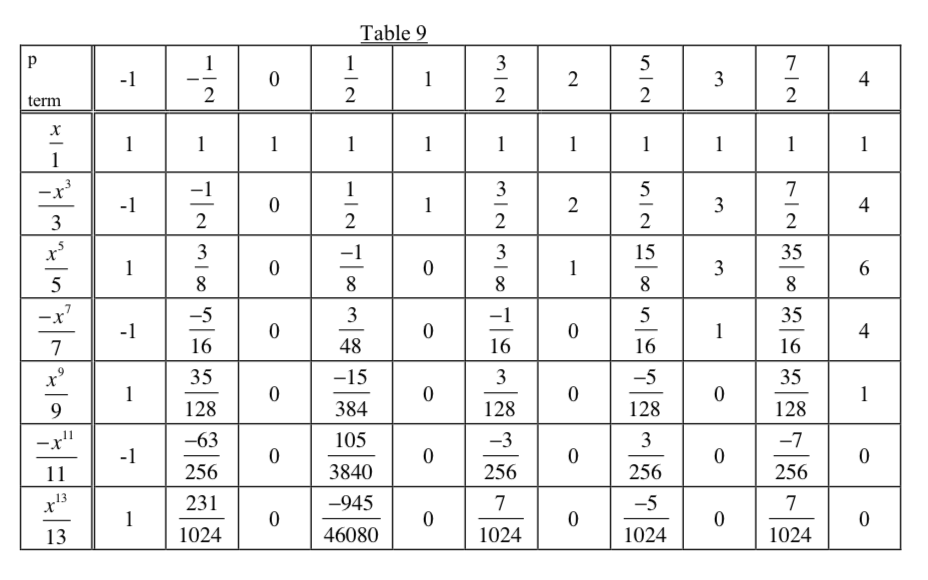
\includegraphics [scale=0.5] {table9.png} \end{center}

Looking at these values, Newton came up with his version of the binomial, which can generate them, and is where we started.

\subsection*{Pi}

\subsection*{Computation of $\pi$}
The series generated under the $1/2$ power is 
\[ x - \frac{1}{4} \ \frac{x^2}{2} + \frac{3}{16} \ \frac{x^3}{3} - \frac{15}{96} \ \frac{x^4}{4}  + \cdots \]
if $x = \sqrt{1-u^2}$, this is

\[ x - \frac{1}{4} \ \frac{x^2}{2} + \frac{3}{16} \ \frac{x^3}{3} - \frac{15}{96} \ \frac{x^4}{4}  + \cdots \]
and it's the area under the quarter-circle ($\pi/4$), when $x=1$.
\[ \frac{\pi}{4} = 1 - \frac{1}{4} \ \frac{1}{2} + \frac{3}{16} \ \frac{1}{3} - \frac{15}{96} \ \frac{1}{4}  \]
\[ = 1 - \frac{1}{8} + \frac{3}{48} - \frac{15}{384} + \cdots  \]

which is a reasonable series for $\pi/4$.

\subsection*{Taylor series}
It's worth mentioning how we would get this series by a modern approach.  Write the general Taylor series
\[ \sum f^n(x - a) \frac{(x-a)^n}{n!} \]
near $a = 0$
\[ \sum f^n(x) \frac{x^n}{n!} \]

The function is 
\[ f(x) = \frac{1}{\sqrt{1 + x}} = (1 + x)^{-1/2} \]
The derivatives are
\[ f'(x) = -\frac{1}{2} (1 + x)^{-3/2} = -\frac{1}{2} \]
\[ f''(x) = \frac{3}{4} (1 + x)^{-5/2} =  \frac{3}{4}  \]
\[ f'''(x) = -\frac{15}{8} (1 + x)^{-7/2} =  -\frac{15}{8}\]
\[ f''''(x) = \frac{105}{16} (1 + x)^{9/2} =  \frac{105}{16} \]

The series is then
\[ 1 -\frac{1}{2} x + \frac{3}{4} \frac{x^2}{2} -\frac{15}{8} \ \frac{x^3}{3!} +  \frac{105}{16} \ \frac{x^4}{4!} + \dots \]
\[ = 1 - \frac{1}{2} x + \frac{3}{8} x^2 - \frac{5}{16} x^3 + \frac{35}{128} x^4 + \dots \]
which matches the table, above.

\end{document}  